\documentclass[11pt,aspectratio=169]{beamer}
%\documentclass[11pt,aspectratio=169,handout]{beamer}

\usepackage{amsmath}
\usepackage{amsfonts}
\usepackage{amssymb}
\usepackage{graphbox}
\usepackage{sgamevar}
\usepackage{pgfplots}
\usepackage{tikz}
\usepackage{pstricks,pst-node}
\usepackage{bigdelim}
\usepackage{qrcode}
\usepackage[absolute,overlay]{textpos}
\usepackage[ruled,vlined]{algorithm2e}



% alg
\SetKwFor{Repeat}{repeat}{}{}
\SetKwComment{Comment}{$\triangleright$ }{}
\SetCommentSty{textsf}
% pgfplot settings
\usepgfplotslibrary{fillbetween}

% tikz settings
\tikzset{
    invisible/.style={text opacity=1,opacity=0},
    visible on/.style={alt=#1{}{invisible}},
    alt/.code args={<#1>#2#3}{%
      \alt<#1>{\pgfkeysalso{#2}}{\pgfkeysalso{#3}}
    },
  }
\newcommand{\nebox}[2][]{\tikz[baseline=(h.base)]\node[rounded corners,rectangle,draw,line width=0.7pt,text depth=-4.9pt,#1] (h) {#2};}
\usetikzlibrary{arrows}
% Customized colors

\definecolor{ashgrey}{rgb}{0.7, 0.75, 0.71}
\definecolor{lightblue}{RGB}{140, 201, 247}
\definecolor{darkgreen}{RGB}{113, 160, 55}
\definecolor{darkblue}{RGB}{78, 103, 200}
\definecolor{darkpurple}{RGB}{112, 48, 160}

% Hyperlink settings

\hypersetup{colorlinks,urlcolor=darkgreen}

%Beamer settings

\setbeamertemplate{navigation symbols}{} 
\setbeamertemplate{footline}[frame number]
\setbeamertemplate{itemize items}[circle]
\setbeamertemplate{section in toc}[sections numbered]
\setbeamertemplate{subsection in toc}[subsection numbered]

\setbeamercolor{section in toc}{fg=blue}

\AtBeginSection[ ]{
 \begin{frame}{Outline}
  \hypersetup{linkcolor=black}
  \tableofcontents[currentsection]
 \end{frame}
}

% Graphics settings

\graphicspath{{../Figures/}}

% PGFPlot settings

\pgfplotsset{compat = newest}

% Gamesvar settings

\setlength{\arrayrulewidth}{0.91pt}
\renewcommand{\gamestretch}{1.68}
\def\stackedpayoffs#1#2{%
 \begin{array}{c}#1\\[2mm]#2\end{array}
}

% Math

\DeclareMathOperator*{\argmax}{argmax}
\DeclareMathOperator*{\argmin}{argmin}

\newcommand\given[1][]{\:#1\vert\:}
\newtheorem{proposition}{Proposition}

% New environments

\newenvironment{itemizes}[1][1em]{
 \vspace{#1}
 \begin{itemize}
 \setlength{\itemsep}{#1}
}{
 \end{itemize}
}


% Shared title frame

\title{Game-theoretic \\ Foundations of Multi-agent Systems}

\author{Seyed Majid Zahedi}
\titlegraphic{\vspace{-4.2em} 
\includegraphics[height=5.8em]{Logos/logo2}}

\date{} 
\subject{Lecture 1} 
\logo{
\includegraphics[height=5.6em]{Logos/logo1}}
\subtitle{\vspace{2.1em}Lecture 9: Learning in Games}

\begin{document}

 \begin{frame}[plain]
  \titlepage
 \end{frame} 
 
 \section{Introduction}
 
  \begin{frame}{Single-agent vs Muli-agent Learning}
   \begin{itemize}[<+->]
   \setlength{\itemsep}{0.7em}
    \item In artificial intelligence (AI), learning is usually performed by \alert{single agent}
    \item Learning agent learns to function successfully in \alert{unknown environment}
    \item In multi-agent setting, environment contains other agents
    \item Agents' learning changes the environment
    \item These changes \alert{depend} in part on actions of learning agents
    \item Learning of each agent is \alert{impacted} by learning performed by others
    \item Different learning rules lead to different \alert{dynamical system}
    \item Simple learning rules can lead to complex global behaviors of system
   \end{itemize}
  \end{frame}
  
  
  \begin{frame}{Learning and Teaching}
   \begin{itemize}[<+->]
   \setlength{\itemsep}{0.5em}
    \item In multi-agent systems, learning and teaching are inseparable
    \item Agents must consider what they have \alert{learned} from others' past behavior
    \item They also must consider how they wish to \alert{influence} others' future behavior
    \item In such setting, learning as \alert{accumulating knowledge} is not always beneficial
    \item Accumulating knowledge should never hurt, one can always ignore what is learned
    \item But when one pre-commits to particular strategy for \\acting on accumulated knowledge, sometimes less is more
    \item E.g., in game of Chicken, if your opponent is learning your strategy to play best response, then optimal strategy is to always dare
   \end{itemize}
  \end{frame}
  
  
  \begin{frame}{Is Agent Learning in Optimal Way?}
   \begin{itemize}[<+->]\small
   \setlength{\itemsep}{0.7em}
    \item In (repeated or stochastic) zero-sum games, this question is meaningful to ask
    \item In general, answer depends not only on learning procedure but also on others' behavior
    \item When all agents adopt same strategy, the setting is called \alert{self-play}
    \begin{itemizes}[0.5em]
     \item  E.g., all agent adopt TfT, or all adopt reinforcement learning (RL)
    \end{itemizes}
    \item One way to evaluate learning procedures is based on their performance in self-play
    \item But learning agents can also be judged by how they do in context of other agent types
    \begin{itemizes}[0.5em]
     \item TfT agent may perform well against TfT agents, but less well against RL agents
    \end{itemizes}
    \item Note that in GT, \alert{optimal strategy} is replaced by \alert{best response} (and equilibrium)
   \end{itemize}
  \end{frame}
  
  
  \begin{frame}{Properties of Learning Rules}
   \begin{itemize}[<+->]
   \setlength{\itemsep}{1.5em}
    \item \alert{Safety}: Guarantee agents at least their maxmin value
    \item \alert{Rationality}: Settle on best response to opponent's strategy whenever opponent settles on stationary strategy
    \begin{itemizes}
     \item Opponent adopts same mixed strategy each time, regardless of the past
    \end{itemizes}
    \item \alert{No regret}: Yield payoff that is no less than payoff agent could have obtained by playing any pure strategy against any set of opponents (details later!)
   \end{itemize}
  \end{frame}
  

 \section{Background}
  
  
  \begin{frame}{Nash Equilibrium}
   \begin{itemize}[<+->]
   \setlength{\itemsep}{0.7em}
    \item \alert{Nash equilibrium (NE)}: No agent wins from unilateral deviation
    $$u_i(s_i^*,s_{-i}^*) \ge u_i(s_i^\prime,s_{-i}^*) ~~~~ \forall i, s_i^\prime$$
    \item \alert{Pure-strategy NE}: NE strategies are pure strategies for all agents
    \begin{itemizes}[0.5em]
     \item It is opposite of \alert{mixed-strategy NE}
    \end{itemizes}
    \item \alert{Strict NE}: Any agent who unilaterally deviates looses
    $$u_i(s_i^*,s_{-i}^*) > u_i(s_i^\prime,s_{-i}^*) ~~~~ \forall i, s_i^\prime\ne s_i^*$$
    \vspace{-1em}
    \begin{itemizes}[0.5em]
     \item It is opposite of \alert{weak NE}
     \item Each agent has unique best response to others
     \item Strict NE is necessarily a pure-strategy NE (why?)
    \end{itemizes}
   \end{itemize}
  \end{frame}
  
  
  \begin{frame}{Nash Equilibrium (cont.)}
   \begin{itemize}[<+->]
   \setlength{\itemsep}{0.7em}
    \item \alert{Strong NE}: No coalition of agents wins by unilateral deviation
    \begin{itemizes}[0.5em]
     \item It is not opposite of weak NE! NE can be both strong and weak, either, or neither!
     \item It implies \alert{Pareto-optimality}
    \end{itemizes}
    \item \alert{Stable NE}: No agent wins by small unilateral deviation, one who deviates loses
    \begin{itemizes}[0.5em]
     \item It is opposite of \alert{unstable NE}
     \item Agents who did not change have no better strategy in the new circumstance
     \item Agent who made a small unilateral change will return immediately to NE
    \end{itemizes}
   \end{itemize}
  \end{frame}
  
  
  \begin{frame}{Nash Equilibrium Beyond Two-player Zero-sum Games}
   \begin{itemize}[<+->]
   \setlength{\itemsep}{1.2em}
    \item NE is invaluable \alert{descriptive} tool in game theory
    \item But NE is problematic as \alert{prescriptive} tool beyond two-player zero-sum game
    \item NE is hard to compute even in two-player general-sum games
    \item Equilibrium selection is challenging (coordination without communication)
   \end{itemize}
  \end{frame}
  
  
  \begin{frame}{Correlated Equilibrium (CE)}
   \begin{columns}
    \begin{column}{0.75\textwidth}
   \begin{itemize}[<+->]
   \setlength{\itemsep}{0.7em}
    \item CE is notion of rationality proposed by Aumann\footnotemark
    \item Agents receive \alert{recommendations} according to distribution
    \item Distribution is CE if agents have no incentives to deviate
    \item It overcomes shortcomings of NE as prescriptive tool
    \item CE does not suffer from equilibrium selection
    \item And, it enables better social welfare
    \item CE arises naturally as empirical frequency of play by independent learners (details later!)
   \end{itemize}
    \end{column}
    \begin{column}{0.3\textwidth}
     \visible<1->{\begin{center}
      \includegraphics<1->[width=0.6\textwidth]{L9/Aumann}\\
      {\scriptsize Robert J. Aumann\footnotemark{}\\(born in 1930)}
     \end{center}}
    \end{column}
   \end{columns}
   \footnotetext[1]{\tiny Aumann, R. J. ``Subjectivity and correlation in randomized strategies.'' 1974}
  \end{frame}
  
  
  \begin{frame}{Correlated Equilibrium  CE (cont.)}
   \begin{itemize}[<+->]
   \setlength{\itemsep}{1.5em}
    \item Distribution $\pi$ over action profiles $A$ is correlated equilibrium if:
    $$\E_{a \sim \pi}[u_i(a)] \geq \E_{a \sim \pi}[u_i(a_i^\prime, a_{-i}) \given a_i]$$\\
    for all $i$ and $a_i^\prime$
    \item After $a$ is drawn, playing $a_i$ is best response for $i$ \alert{after} seeing $a_i$, given that everyone else plays according to $a$
   \end{itemize}
  \end{frame}
  
  
  \begin{frame}{Coarse Correlated Equilibrium}
   \begin{itemize}[<+->]
   \setlength{\itemsep}{1em}
    \item Distribution $\pi$ over action profiles $A$ is coarse correlated equilibrium if:
    $$\E_{a \sim \pi}[u_i(a)] \geq \E_{a \sim \pi}[u_i(a_i^\prime, a_{-i})]$$\\
    for all $i$ and $a_i^\prime$
    \item After $a$ is drawn, playing $a_i$ is best response for $i$ \alert{before} seeing $a_i$, given that everyone else plays according to $a$
    \item This makes sense if agents have to commit \alert{up front} to following recommendations or not (deviations are not allowed after recommendations are received)
    \item Coarse correlated equilibrium could occasionally recommend really bad actions!
   \end{itemize}
  \end{frame}
  
  
  \begin{frame}{Coarse Correlated Equilibrium: Example}
   \begin{center}\scriptsize
   \renewcommand{\gamestretch}{2.5}
    \hspace{-3.2em}
    \begin{game}{3}{3}
         \> A								\> B     							\> C											\\
     A   \> $\stackedpayoffs{1, 1}{33.3\%}$	\> $\stackedpayoffs{-1, -1}{0\%}$		\> $\stackedpayoffs{0, 0}{0\%}$				\\
     B   \> $\stackedpayoffs{-1,  -1}{0\%}$	\> $\stackedpayoffs{1,  1}{33.3\%}$	\> $\stackedpayoffs{0, 0}{0\%}$				\\
     C   \> $\stackedpayoffs{0,  0}{0\%}$		\> $\stackedpayoffs{0,  0}{0\%}$		\> $\stackedpayoffs{-1.1, -1.1}{33.3\%}$	\\
    \end{game}
   \end{center}
   \vspace{1em}
   \begin{itemize}[<+->] \footnotesize
    \item Utility for following $\pi$: $1/3 + 1/3 - 1.1/3 = 0.3$
    \item Utility for playing $A$ or $B$ if other agent follows $\pi$: $1/3 - 1/3 + 0 = 0$
    \item Utility for playing $C$ is strictly less than zero
    \item $\pi$ \alert{is coarse correlated} equilibrium 
    \item But, if recommendation is $C$, it is not best response to play $C$ (why?)
    \item Therefore, $\pi$ \alert{is not correlated equilibrium}
   \end{itemize}
  \end{frame}
  
  
  \begin{frame}{Equilibrium Notions for Normal-form Games}
   \begin{itemizes}
    \item Dominant strategy equilibria (DSE)
    \item Pure strategy Nash equilibria (PSNE)
    \item Mixed strategy Nash equilibria (MSNE)
    \item Correlated equilibria (CE)
    \item Coarse correlated equilibria (CCE)
    \item<2-> DSE $\subseteq$ PSNE $\subseteq$ MSNE $\subseteq$ CE $\subseteq$ CCE
    \item<3-> In two-player zero-sum games, CE = CCE = NE 
   \end{itemizes}
  \end{frame}
  
  
 \section{Fictitious Play}
  
  \begin{frame}{Fictitious Play: Introduction}
   \begin{itemize}[<+->]
   \setlength{\itemsep}{1.2em}
    \item What are agents learning about?
    \item Arguably, most plausible answer is strategies of others
    \item \alert{Fictitious} play (FP), one of earliest learning rules, takes this approach
    \item FP was first introduced by G. W. Brown in 1951%
    \footnote{\tiny Brown, G. W. ``Iterative solution of games by fictitious play.'' 1951}
    \item Brown imagined that agents would \alert{``simulate''} the game in their mind and update their future play based on this simulation; hence name fictitious play
    \item In its current use, FP is misnomer, since each play of the game actually occurs
   \end{itemize}
  \end{frame}
  
  
  \begin{frame}{Fictitious Play}
   \begin{itemize}[<+->]
    \item Two agents repeatedly play stage game $G$
    \item $\eta_i^t(a_{-i})$ denotes number of times agent $i$ has observed $a_{-i}$ before time $t$
    \item $\eta_i^1$ represents \alert{fictitious past} and cannot be zero for all $a_{-i}$
    \item Agents assume that their opponent is using \alert{stationary mixed strategy}
    \item Agents \alert{update their beliefs} about this strategy at each step according to:
    $$\mu_i^t(a_{-i})=\frac{\eta_i^t(a_{-i})}{\sum_{a_{-i}^\prime}\eta_i^t(a_{-i}^\prime)}$$
    \item $\mu_i^t$ is \alert{empirical distribution} of past actions and is treated as mixed strategy
    \item Agents best-respond to their beliefs about opponent' strategy
    $$a_i^{t+1}=\underset{a_i}{\argmax}~u_i(a_i,\mu_i^t)$$
   \end{itemize}
  \end{frame}
  
  
  \begin{frame}{Fictitious Play: Example}
   \begin{itemize}[<+->]
    \item Consider the following coordination game
    \begin{center}\scriptsize
     \hspace{-3.5em}
     \begin{game}{2}{2}
      	\> L		\> R		\\
      U	\> $3,3$	\> $0,0$	\\
      D	\> $4,0$	\> $1,1$
     \end{game}
    \end{center}
    \vspace{1em}
    \item Note that this game is dominant solvable with unique NE of (D, R)
    \item Suppose that $\eta_1^1 = (3, 0)$ and $\eta_2^1 = (1, 2.5)$
    \item FP proceeds as follows:
    \vspace{1em}
    \begin{center}
     \begin{tabular}{ccccc}
      Round	& 1's $\eta$	& 2's $\eta$	& 1's action	& 2's action			\\ \hline
      1		& (3, 0)		& (1, 2.5) 	& D			& L			\pause	\\
      2		& (4, 0)		& (1, 3.5) 	& D			& R			\pause	\\
      3		& (4, 1)		& (1, 4.5) 	& D			& R			\pause	\\
      4		& (4, 2)		& (1, 5.5) 	& D			& R					\\
     \end{tabular}
    \end{center}
   \end{itemize}
  \end{frame}
  
  
  \begin{frame}{Fictitious Play: Discussion}
   \begin{itemize}[<+->]
   \setlength{\itemsep}{1.2em}
    \item In FP, agents \alert{do not} need to know anything about their opponent's utilities
    \item FP is somewhat paradoxical as agents assume stationary strategy for their opponent, yet no agent plays stationary strategy except when FP converges
    \item Even though FP is \alert{belief based} it is also \alert{myopic}
    \item I.e., agents maximize current utility without considering their future ones
    \item Agents do not learn \alert{true model} that generates empirical frequencies
    \item In other words, they do not learn how their opponent is actually playing the game
   \end{itemize}
  \end{frame}
  
  
  \begin{frame}{Convergence of Fictitious Play to Pure Strategies}
   \begin{itemize}[<+->]
   \setlength{\itemsep}{1.2em}
    \item Let $\{a^t\}$ be sequence of action profiles generated by FP for $G$
    \item Sequence \alert{converges} to $a^*$ if there exists $T$ s.t. $a^t = a^*$ for all $t\ge T$
    \item $a^*$ is called \alert{steady state} or \alert{absorbing state} of FP
    \item (I) If sequence converges to $a^*$, then $a^*$ is pure-strategy NE of $G$
    \item (II) If for some $t$, $a^t = a^*$, where $a^*$ is strict NE of $G$, then $a^\tau = a^*$ for all $\tau > t$
   \end{itemize}
  \end{frame}
  
  
  \begin{frame}{Proof}
   \begin{itemize}[<+->]
    \item (I) is straightforward, for (II), let $a^t = a^*$, we want to show that $a^{t+1} = a^*$
    \item First, note that we can write $\mu$ as: 
    $$\mu_i^{t+1} = (1-\alpha)\mu_i^t + \alpha a_{-i}^t = (1-\alpha)\mu_i^t + \alpha a^*_{-i}$$
    here, abusing notation, $a_{-i}^t$ denotes degenerate probability distribution and:
    $$\alpha = \frac{1}{\sum_{a_{-i}^\prime}\eta_i^t(a_{-i}^\prime)+1}$$
    \item By linearity of expected utility, we have for all $a_i$:
    $$u_i(a_i,\mu_i^{t+1}) = (1-\alpha)u_i(a_i,\mu_i^t)+\alpha u_i(a_i,a_{-i}^*)$$
    \item Since $a_i^*$ maximizes both terms, it follows that it is played at $t+1$
   \end{itemize}
  \end{frame}
  
  
  \begin{frame}{Convergence of Fictitious Play to Mixed Strategies}
   \begin{itemize}[<+->]
   \setlength{\itemsep}{0.7em}
    \item Of course, one cannot guarantee that fictitious play always converges to NE
    \item In FP, agents only play pure strategies and pure-strategy NE may not exist
    \item While FP sequence may not converge, its empirical distribution may
    \item Sequence $\{a^t\}$ converges to $s^*$ in time-average sense if for all $i$ and $a_i$:
    $$\lim_{T\to\infty}\frac{\sum_{t=1}^{T}\mathds{1}(a_i^t=a_i)}{T} = s^*_i(a_i)$$
    $\mathds{1}(\cdot)$ denotes the indicator function
    \item If FP sequence converges to $s^*$ in the time-average sense, then $s^*$ is NE
   \end{itemize}
  \end{frame}
  
  
  \begin{frame}{Proof}
   \begin{itemize}[<+->]
   \setlength{\itemsep}{1.2em}
    \item Suppose $\{a^t\}$ converges to $s^*$ in time-average sense, but $s^*$ is not NE
    \item There is some $i$, $a_i^\prime$, and $a_i$ with $s_i^*(a_i)>0$ s.t. $u_i(a_i^\prime,s_{-i}^*)>u_i(a_i,s_{-i}^*)$
    \item Choose $\epsilon$ s.t. $\epsilon < \left(u_i(a_i^\prime,s_{-i}^*) - u_i(a_i,s_{-i}^*)\right)/2$
    \item Choose $T$ s.t. for all $t\ge T$, $\vert \mu_i^t(a_{-i}) - s_{-i}^*(a_{-i}) \vert < \epsilon/\max_{a^\prime} u_i(a^\prime)$ for all $a_{-i}$
    \item This is possible because $\mu_i^t(a_{-i})\to s_{-i}^*(a_{-i})$ by assumption
   \end{itemize}
  \end{frame}
  
  
  \begin{frame}{Proof (cont.)}
   \begin{itemize}
    \item<1-> Then, for any $t \ge T$, we have:
    \begin{eqnarray*}
     u_i(a_i, \mu_i^t) & = & \sum_{a_{-i}}u_i(a_i, a_{-i})\mu_i^t(a_{-i}) \\ \pause
     & \le & \sum_{a_{-i}}u_i(a_i, a_{-i})s_{-i}^*(a_{-i}) + \epsilon \\ \pause
     & \le & \sum_{a_{-i}}u_i(a_i^\prime, a_{-i})s_{-i}^*(a_{-i}) - \epsilon \\ \pause
     & \le & \sum_{a_{-i}}u_i(a_i^\prime, a_{-i})\mu_i^t(a_{-i}) = u_i(a_i^\prime, \mu_i^t) \\ \pause
    \end{eqnarray*}
    \vspace{-2em}
    \item<5-> So after sufficiently large $t$, $a_i$ is never played
    \item<6-> This implies that as $t \to \infty$, $\mu_i^t(a_i)\to 0$, which contradicts with $s_i^*(a_i) > 0$
   \end{itemize}
  \end{frame}
  
  
  \begin{frame}{Example: Matching Pennies}
   \begin{itemize}[<+->]
    \item Consider the matching-pennies game
    \begin{center}\scriptsize
     \hspace{-3.5em}
     \begin{game}{2}{2}
      	\> H			\> T		\\
      H	\> $1,-1$	\> $-1,1$	\\
      T	\> $-1,1$	\> $1,-1$
     \end{game}
    \end{center}
    \vspace{0.75em}
    \begin{center}
     \begin{tabular}{ccccc}
      Round	& 1's $\eta$	& 2's $\eta$	& 1's action	& 2's action			\\ \hline
      1		& (1.5, 2)	& (2, 1.5) 	& T			& T			\pause	\\
      2		& (1.5, 3)	& (2, 2.5) 	& T			& H			\pause	\\
      3		& (2.5, 3)	& (2, 3.5) 	& T			& H			\pause	\\
      4		& (3.5, 3)	& (2, 4.5) 	& H			& H			\pause	\\
      5		& (4.5, 3)	& (3, 4.5) 	& H			& H			\pause	\\
      6		& (5.5, 3)	& (4, 4.5) 	& H			& H			\pause	\\
      7		& (6.5, 3)	& (5, 4.5) 	& H			& T			\pause	\\
     \end{tabular}
    \end{center}
    \vspace{0.75em}
    \item FP continues as deterministic cycle, time average converges to unique NE
   \end{itemize}
  \end{frame}
  
  
  \begin{frame}{Example: (Anti-)Coordination Game}
   \begin{itemize}[<+->]
    \item Note that if empirical distribution of actions converges to NE, there is no guarantee on distribution of played outcomes
    \item Consider the following coordination game
    \begin{center}\scriptsize
     \hspace{-3.5em}
     \begin{game}{2}{2}
      	\> A		\> B		\\
      A	\> $1,1$	\> $0,0$	\\
      B	\> $0,0$	\> $1,1$
     \end{game}
    \end{center}
    \vspace{1em}
    \item Note that this game is unique NE of ((0.5, 0.5), (0.5, 0.5))
    \vspace{1em}
    \begin{center}
     \begin{tabular}{ccccc}
      Round	& 1's $\eta$	& 2's $\eta$	& 1's action	& 2's action			\\ \hline
      1		& (0.5, 0)	& (0, 0.5) 	& A			& B			\pause	\\
      2		& (0.5, 1)	& (1, 0.5) 	& B			& A			\pause	\\
      3		& (1.5, 1)	& (1, 1.5) 	& A			& B			\pause	\\
      4		& (1.5, 2)	& (2, 1.5) 	& B			& A					\\
     \end{tabular}
    \end{center}
   \end{itemize}
  \end{frame}  
  
  
  \begin{frame}{General Fictitious Play Convergence}
   \begin{itemize}[<+->]
   \setlength{\itemsep}{1.2em}
    \item Fictitious play converges in time-average sense for game $G$ if:
    \begin{itemizes}
     \item $G$ is zero-sum game
     \item $G$ is two-player game where each agent has at most two actions (2x2 games)
     \item $G$ is solvable by iterated strict dominance
     \item $G$ is \alert{identical-interest game}, i.e., all agents have same payoff function
     \item $G$ is \alert{potential game} (more on this later!)
    \end{itemizes}
   \end{itemize}
  \end{frame}
  
  
  \begin{frame}{Non-convergence of Fictitious Play}
   \begin{itemize}[<+->]
    \item Convergence of fictitious play \alert{can not} be guaranteed in general
    \item Shapley showed that in modified rock-scissors-paper game, FP does not converge
    \vspace{1em}
    \begin{center}\scriptsize
     \hspace{-4.9em}
     \begin{game}{3}{3}
      			\> Rock	\> Paper	\> Scissors	\\
      Rock		\> $0,0$	\> $0,1$	\> $1,0$		\\
      Paper		\> $1,0$	\> $0,0$	\> $0,1$		\\
      Scissors	\> $0,1$	\> $1,0$	\> $0,0$
     \end{game}
    \end{center}
    \vspace{1em}
    \item This game has unique NE: each agent mixes uniformly
    \item Suppose $\eta_1^1=(1,0,0)$ and $\eta_2^1=(0,1,0)$
    \item Shapley showed that play cycles among 6 (off-diagonal) profiles with periods of ever-increasing length, thus non-convergence
   \end{itemize}
  \end{frame}
  
  
  \begin{frame}{Smooth Fictitious Play (SFP)}
   \begin{itemize}[<+->]
   \setlength{\itemsep}{0.7em}
    \item Instead of best-responding to beliefs, agents respond randomly, but somewhat proportional to their expected utility
    $$s_i^t(a_i \given \mu_i^t) = \frac{\exp(u_i(a_i,\mu_i^t)/\gamma)}{\sum_{a_i^\prime}\exp(u_i(a_i^\prime,\mu_i^t)/\gamma)}$$
    \item $\gamma$ is called the \alert{smoothing} parameter
    \item This is called \alert{soft-max} policy
    \item Soft-max policy respects best replies, but leaves room for \alert{exploration}
    \item If all agents use SFP with sufficiently small $\gamma_i$, empirical play converges to $\epsilon$-CCE
   \end{itemize}
  \end{frame}
  
 
 \section{Best-response Dynamics}  
  
  \begin{frame}{Best-response Dynamics (BRD): Introduction}
   \begin{itemize}[<+->]
    \item Agents start playing \alert{arbitrary} actions
    \item In arbitrary order, agents take turns updating their action
    \item Agent update their action only if doing so can improve their utility
    \item This is repeated until no agents wants to update their action
   \end{itemize}
   \vspace{1em}
   \visible<4>{\begin{algorithm*}[H]
    Initialize $a = (a_1,\dots,a_n)$ to be arbitrary action profile\;
    \While{there exists $i$ such that $a_i \not\in \argmax_{a \in A_i}u_i(a,a_{-i})$}{
     Let $a_i^\prime$ be such that $u_i(a_i^\prime, a_{-i}) > u(a)$\;
     Set $a_i \leftarrow a_i^\prime$\;
    }
    \Return $a$
   \end{algorithm*}}
  \end{frame}
  
  
  \begin{frame}{Best-response Dynamics: Discussion}
   \begin{itemize}[<+->]
   \setlength{\itemsep}{1.5em}
    \item If BRD halts, it returns pure strategy Nash equilibrium
    \begin{itemizes}
     \item Every agent must be playing best response
    \end{itemizes}
    \item Does BRD always halt?
    \begin{itemizes}
     \item No: Consider matching pennies/Rock Paper Scissors
    \end{itemizes}
   \end{itemize}
  \end{frame}
  
  
  \begin{frame}{Example: Congestion Games}
   \begin{itemize}[<+->]
   \setlength{\itemsep}{0.7em}
    \item $N$ is set of $n$ agents
    \item $M$ is set of $m$ \alert{resources}
    \item $A_i$ is set of actions available to agent $i$
    \begin{itemize}
     \item $a_i$ represents subset of resources that agent $i$ chooses (i.e., $a_i \subseteq M$)
    \end{itemize}
    \item $\ell_j$ is \alert{congestion cost function} for resources $j \in M$
    \begin{itemize}
     \item $\ell_j(k)$ represents cost of congestion on resource $j$ when $k$ agents choose $j$
    \end{itemize}
    \item $n_j(a)$ is number of agents who choose resource $j$ (i.e., $n_j(a) = \vert\{i \given j \in a_i\}\vert$)
    \item $c_i(a) = \sum_{j \in a_i} \ell_j(n_j(a))$ is total cost of agent
    \item Agents minimize their total cost (instead of maximizing their total utility)
   \end{itemize}
  \end{frame}
  
  
  \begin{frame}{BRD in Congestion Games}
   \begin{itemize}
    \item<1-> Consider \alert{potential function}  $\phi:A\rightarrow \R$:
    $$\phi(a) = \sum_{j=1}^m \sum_{k=1}^{n_j(a)} \ell_j(k)$$
    (Note: \alert{not} social welfare)
    \item<2-> How does $\phi$ change in one round of BRD? Say $i$ switches from $a_i$ to $b_i \in A_i$
    \item<3->Well... We know it must have decreased agent $i$'s cost:
    \begin{eqnarray*}
     \Delta c_i & \equiv & c_i(b_i, a_{-i}) - c_i(a_i, a_{-i}) \\ 
     & = & \sum_{j \in b_i\setminus a_i}\ell_j(n_j(a)+1) - \sum_{j \in a_i \setminus b_i}\ell_j(n_j(s)) < 0
    \end{eqnarray*}
   \end{itemize}
  \end{frame}
  
  
  \begin{frame}{BRD in Congestion Games (cont.)}
   $$\phi(a) = \sum_{j=1}^m \sum_{k=1}^{n_j(a)} \ell_j(k)$$
   \begin{itemize}[<+->]
    \item Change in potential is:
    \begin{eqnarray*}
     \Delta\phi & \equiv & \phi(b_i, a_{-i}) - \phi(a_i, a_{-i}) \\
     & = & \sum_{j \in b_i\setminus a_i}\ell_j(n_j(a)+1) - \sum_{j \in a_i \setminus b_i}\ell_j(n_j(s)) \\
     & = & \Delta c_i
    \end{eqnarray*}
    \item Since $\phi$ can take on only finitely many values, this cannot go on forever
    \item And hence BRD halts in congestion games ...
    \item Which proves the \alert{existence} of pure strategy Nash equilibria!
   \end{itemize}
  \end{frame}
  
  
  \begin{frame}{Example: Load Balancing Games on Identical Servers}
   \begin{itemize}[<+->]
   \setlength{\itemsep}{1.5em}
    \item $n$ clients $i \in N$ schedule jobs of size $w_i > 0$ on $m$ identical servers $M$
    \item Action space $A_i = M$ for each client
    \item For each server $j \in M$, load $\ell_j(a) = \sum_{i : a_i = j}w_i$
    \item Cost of client $i$ is load of server that $i$ chooses : $c_i(a) = \ell_{a_i}(a)$
   \end{itemize}
  \end{frame}
  
  
  \begin{frame}{Load Balancing Games on Identical Servers: Discussion}
   \begin{itemize}[<+->]
   \setlength{\itemsep}{1.5em}
    \item \textit{Almost} congestion game --- but server costs depend on \alert{which} clients choose them
    \item BRD converges in load balancing games on identical servers
    \item Load balancing games on identical servers have pure strategy NE
   \end{itemize}
  \end{frame}
  
  
  \begin{frame}{BRD in Load Balancing Games on Identical Servers}
   \begin{itemize}
    \item Consider \alert{potential function} $\phi$ as:
    $$\phi(a) = \frac{1}{2}\sum_{j=1}^m\ell_j(a)^2$$
    \item Suppose $i$ switches from server $j$ to server $j'$:
    \begin{eqnarray*}
     \Delta c_i(a) & \equiv & c_i(j', a_{-i}) - c_i(j, a_{-i}) \\ \pause
     & = & \ell_{j'}(a) + w_i - \ell_j(a) \\ \pause 
     & < & 0
    \end{eqnarray*}
   \end{itemize}
  \end{frame}


  \begin{frame}{BRD in Load Balancing Games on Identical Servers (cont.)}
   \begin{center}
    \begin{eqnarray*}
     \Delta \phi(a) & \equiv & \phi(j', a_{-i}) - \phi(j, a_{-i}) \\ \pause
     & = & \frac{1}{2}\left((\ell_{j'}(a)+w_i)^2 + (\ell_j(a)-w_i)^2 - \ell_{j'}(a)^2 - \ell_j(a)^2  \right) \\ \pause
     & = & \frac{1}{2}\left(2w_i\ell_{j'}(a) + w_i^2 -2w_i\ell_j(a) + w_i^2  \right) \\ \pause
     & = & w_i\left(\ell_{j'}(a) + w_i - \ell_j(a)  \right) \\ \pause
     & = & w_i\cdot \Delta c_i(a) \\ \pause 
     & < & 0
    \end{eqnarray*}
    \pause
    \hspace{-8cm}
    \alert{Note: $\Delta c_i \neq \Delta \phi$}
   \end{center}
  \end{frame}
  
  
  \begin{frame}{Potential Games}
   \begin{itemize}[<+->]
   \setlength{\itemsep}{1.2em}
    \item $\phi:A\rightarrow \R_{\geq 0}$ is \alert{exact potential function} for game $G$ if for all $a$, $i$,$a_i$, and $b_i$:
    $$\phi(b_i, a_{-i}) - \phi(a_i, a_{-i}) = c_i(b_i, a_{-i}) - c_i(a_i,a_{-i})$$
    \item $\phi:A\rightarrow \R_{\geq 0}$ is \alert{ordinal potential function} for game $G$ if for all $a$, $i$,$a_i$, and $b_i$:
    $$(c_i(b_i, a_{-i}) - c_i(a_i,a_{-i}) < 0) \Rightarrow (\phi(b_i, a_{-i}) - \phi(a_i, a_{-i}) < 0)$$
    (i.e. the change in utility is always equal \alert{in sign} to the change in potential)
    \item BRD is \alert{guaranteed} to converge in game $G$ \alert{iff} $G$ has ordinal potential function
   \end{itemize}
  \end{frame}
  
  
  \begin{frame}{BRD and Potential Games}
   \begin{itemize}[<+->]
   \setlength{\itemsep}{0.7em}
    \item We've already seen ordinal potential function $\Rightarrow$ BRD converges
    \item Lets prove other direction
    \item Consider graph $G = (V,E)$
    \item Let each $a \in A$ be a vertex in $G$ (i.e., $V = A$)
    \item Add directed edge $(a,b)$ if it is possible to go from $b$ to $a$ by best-response move
    \begin{itemize}
     \item I.e., if there is $i$ such that $b = (b_i, a_{-i})$, and $c_i(b_i, a_{-i}) < c_i(a)$
    \end{itemize}
    \item BRD can be viewed as traversing this graph
    \begin{itemize}
     \item Start at arbitrary vertex $a$, and then traverse arbitrary outgoing edges
    \end{itemize}
   \end{itemize}
  \end{frame}


  \begin{frame}{BRD and Potential Games (cont.)}
   \begin{itemize}[<+->]
   \setlength{\itemsep}{0.7em}
    \item Nash Equilibria are the sinks in this graph
    \item Suppose BRD converges $\Rightarrow$ there are no cycles in this graph
    \item So, from every vertex $a$ there is some sink $s$ that is reachable (why?)
    \item We construct potential function $\phi(a)$ for each vertex $a$
    \item $\phi(a)$ is length of \alert{longest} finite path from $a$ to any sink $s$
    \item We need: for any edge $a \rightarrow b$, $\phi(b) < \phi(a)$.
    \item Its true! $\phi(a) \geq \phi(b) + 1$. (why?)
   \end{itemize}
  \end{frame}
  
  
 \section{No-regret Learning}
  
  \begin{frame}{Sequential Prediction: Stock-prediction Example}
   \begin{itemize}[<+->]
   \setlength{\itemsep}{1.2em}
    \item Every day GME goes \alert{up} or \alert{down}
    \item Goal is to predict direction each day before market opens (to buy or short)
    \item Market can behave arbitrarily/adversarially
    \item So there is no way we can promise to do \alert{well}
    \item However, we get \alert{advice}
   \end{itemize}
  \end{frame}
  
  
  \begin{frame}{Expert Advice}
   \begin{itemize}[<+->]
   \setlength{\itemsep}{1em}
    \item There are $N$ \alert{experts} who make predictions in $T$ rounds
    \item At each round $t$, each expert $i$ makes prediction $p_i^t \in \{U, D\}$
    \item Expertise is self proclaimed --- no promise experts know what they're talking about
    \item We (algorithm) want to aggregate predictions, to make our own prediction $p_A^t$
    \item We learn true outcome $o^t$ at the end of each round
    \item If we predicted incorrectly (i.e. $p_A^t \neq o^t$), then we \alert{made a mistake}
   \end{itemize}
  \end{frame}
  
  
  \begin{frame}{Expert Advice (cont.)}
   \begin{itemize}[<+->]
   \setlength{\itemsep}{1em}
    \item Goal is to after a while do (almost) as well as \alert{best} expert in hindsight
    \item To make things easy, we assume for now that there is one \alert{perfect} expert
    \item Perfect expert never makes mistakes (but we don't know who the expert is)
    \item Can we find strategy that is guaranteed to make at most $\log(N)$ mistakes?
   \end{itemize}
  \end{frame}
  
  
  \begin{frame}{The Halving Algorithm}
   \begin{algorithm*}[H]
    Let $S^1 \leftarrow \{1,\ldots,N\}$ be set of all experts\;
    \For{$t = 1$ to $T$}{
     Predict with majority vote\;
     Observe the true outcome $o^t$\;
     Eliminate all experts that made a mistake: $S^{t+1} = \{i \in S^t \given p_i^t = o^t\}$\;
    }
   \end{algorithm*}
  \end{frame}
  
  
  \begin{frame}{The Halving Algorithm: Analysis}
   \begin{itemize}[<+->]
   \setlength{\itemsep}{0.7em}
    \item Algorithm predicts with majority vote
    \item Every time it makes a mistake, at least half of remaining experts are eliminated
    \item Hence $|S^{t+1}| \leq |S^t|/2$
    \item On the other hand, perfect expert is never eliminated
    \item Hence $|S^t| \geq 1$ for all $t$
    \item Since $|S^1| = N$, this means there can be at most $\log N$ mistakes
    \item But what if no expert is perfect? Say the best expert makes $\OPT$ mistakes
    \item Can we find a way to make not too many more than $\OPT$ mistakes?
   \end{itemize}
  \end{frame}
  
  
  \begin{frame}{The Iterated Halving Algorithm}
   \begin{algorithm*}[H]
    Let $S^1 \leftarrow \{1,\ldots,N\}$ be the set of all experts\;
    \For{$t = 1$ to $T$}{
     \If{$|S^t| = 0$}{Reset: Set $S^t \leftarrow \{1,\ldots,N\}$}
     Predict with majority vote\;
     Eliminate all experts that made a mistake: $S^{t+1} = \{i \in S^t \given p_i^t = o^t\}$\;
    }
   \end{algorithm*}
  \end{frame}
  
  
  \begin{frame}{The Iterated Halving Algorithm: Analysis}
   \begin{itemize}[<+->]
   \setlength{\itemsep}{0.7em}
    \item Whenever algorithm makes mistake, we eliminate half of experts
    \item So algorithm can make at most $\log N$ mistakes between any two resets
    \item But if we reset, it is because since last reset, \alert{every} expert has made mistake
    \item In particular, between any two resets, \alert{best} expert has made at least 1 mistake
    \item Algorithm makes at most $\log(N)(\OPT + 1)$ mistakes
    \item Algorithm is wasteful in that every time we reset, we forget what we have learned!
    \item How about just \alert{downweight} experts who make mistakes?
   \end{itemize}
  \end{frame}
  
  
  \begin{frame}{The Weighted Majority Algorithm}
   \begin{algorithm*}[H]
    Set weights $w_i^1 \leftarrow 1$ for all experts $i$\;
    \For{$t = 1$ to $T$}{
     Predict with weighted majority vote\;
     Down-weight experts who made mistakes: (i.e., if $p_i^t \neq o^t$, set $w_i^{t+1} \leftarrow w_i^t/2$)
    }
   \end{algorithm*}
  \end{frame}
  
  
  \begin{frame}{The Weighted Majority Algorithm: Analysis}
   \begin{itemize}[<+->]\small
   \setlength{\itemsep}{0.7em}
    \item Let $M$ be total number of mistakes that algorithm makes
    \item Let $W^t = \sum_i w_i^t$ be total weight at step $t$
    \item When algorithm makes mistake, at least half of total weight is cut in half 
    \item So: $W^{t+1} \leq (3/4)W^t$
    \item If algorithm makes $M$ mistakes, $W^T \leq N\cdot(3/4)^M$
    \item Let $i^*$ be the best expert, $W^T > w_i^T = (1/2)^{\OPT}$, which gives:
    $$(1/2)^{\OPT} \leq W \leq N(3/4)^M \Rightarrow (4/3)^M \leq N\cdot 2^\OPT \Rightarrow M \leq 2.4(\OPT + \log(N))$$
    \item Algorithm makes at most $2.4\left(\OPT + \log(N)\right)$ mistakes
    \item $\log(N)$ is constant, so ratio of mistakes to $\OPT$ is $2.4$ in limit -- not great, but not bad
   \end{itemize}
  \end{frame}
  
  
  \begin{frame}{What Do We Want in an Algorithm?}
   \begin{itemizes}[1.5em]
    \item Make only 1$\times$ as many mistakes as $\OPT$ in limit, rather than 2.4$\times$
    \item Handle $N$ distinct actions (separate action for each expert), not just up and down
    \item Handle arbitrary costs in $[0,1]$ per expert per round, not just right and wrong
   \end{itemizes}
  \end{frame}
  
  
  \begin{frame}{New Model/Algorithm}
   \begin{itemize}[<+->]
   \setlength{\itemsep}{1em}
    \item In rounds $1,\ldots, T$, algorithm \alert{chooses some expert} $i^t$
    \item Each expert $i$ \alert{experiences loss}: $\ell_i^t \in [0,1]$
    \item Algorithm experiences the loss of the expert it chooses: $\ell_A^t = \ell_{i^t}^t$
    \item Total loss of expert $i$ is $L_i^T = \sum_{t=1}^T \ell_i^t$
    \item Total loss of algorithm is $L_A^T = \sum_{t=1}^T \ell_A^t$
    \item Goal is to obtain loss \alert{``not much worse''} than that of the best expert: $\min_i L_i^T$
   \end{itemize}
  \end{frame}
  
  
  \begin{frame}{Multiplicative Weights (MW) Algorithm (a.w.a. Hedge Algorithm)}
   \begin{algorithm*}[H]
    Set weights $w_i^1 \leftarrow 1$ for all experts $i$\;
    \For{$t = 1$ to $T$}{
     Let $W^t = \sum_{i=1}^N w_i^t$\;
     Choose expert $i$ with probability $w_i^t/W^t$\;
     For each $i$, set $w_i^{t+1} \leftarrow w_i^t \cdot \exp(-\epsilon \ell_i^t)$\;
    }
   \end{algorithm*}
   
   \vspace{1em}
   
   \begin{itemizes}[0.7em]\small
    \item<2-> Can be viewed as ``smoothed'' version of weighted majority algorithm
    \item<3-> Has parameter $\epsilon$ which controls how quickly it down-weights experts
    \item<4-> Is \emph{randomized} --- chooses experts w.p. proportional to their weights
    \item<5-> Can be used with alternative update: $w_i^{t+1} \leftarrow w_i^t \cdot(1-\epsilon \ell_i^t)$
   \end{itemizes}
  \end{frame}
  
  
  \begin{frame}{Multiplicative Weights Algorithm: Discussion}
   \begin{itemize}[<+->]
    \item For any sequence of losses, and any expert $k$:
    $$\frac{1}{T}~\E[L_{MW}^T] \leq \frac{1}{T}~L_k^T + \epsilon + \frac{\ln(N)}{\epsilon\cdot T}$$
    \item In particular, setting $\epsilon = \sqrt{\ln(N)/T}$:
    $$\frac{1}{T}~\E[L_{MW}^T] \leq \frac{1}{T}~\min_k L_k^T + 2\sqrt{\frac{\ln(N)}{T}}$$
    \item Average loss quickly approaches that of best expert \alert{exactly}, at rate of $1/\sqrt{T}$
    \item This works for \alert{arbitrary} sequence of losses (e.g., chosen adaptively by adversary)
    \item So we could us it to play games (\alert{experts $\leftrightarrow$ actions} and \alert{losses $\leftrightarrow$ costs})
   \end{itemize}
  \end{frame}
  
  
  \begin{frame}{Recall: Minimax Theorem (John von Neumann, 1928)}
   \begin{center}
    In any finite, two-player, zero-sum game, in any NE, each agent receives a payoff that is equal to both their maxmin value and their minmax value
    $$\underset{s_i}{\max} \; \underset{s_{-i}}{\min} \; u_i(s_i,s_{-i}) = \underset{s_{-i}}{\min} \; \underset{s_{i}}{\max} \; u_{i}(s_i,s_{-i})$$
   \end{center}
  \end{frame}
  
  
  \begin{frame}{Simple Proof for Minimax Theorem}
   \begin{itemize}[<+->]
   \setlength{\itemsep}{1em}
    \item Scale utilities such that $u_1$ is in $[0, 1]$
    \item Write $v_1 = \min_{s_{2}} \max_{s_1} u_1(s_1,s_{2})$ and $v_2 = \max_{s_1} \min_{s_{2}} u_1(s_1,s_2)$
    \item Suppose theorem were false: $v_1 = v_2 + \epsilon$ for some constant $\epsilon > 0$
    \item Suppose A1 and A2 repeatedly play against each other as follows
    \begin{itemizes}[0.7em]
     \item A2 uses MW algorithm: at round $t$, $s^t_2(a_2) = w^t_{a_2}/W^t$
     \item A1 plays best response to A2's strategy: $s_1^t = \argmax_{s_1} u_1(s_1, s_2^t)$
    \end{itemizes}
   \end{itemize}
  \end{frame}
  
  
  \begin{frame}{Simple Proof for Minimax Theorem (cont.)}
   \begin{itemize}[<+->]\small
    \item For A2's MW algorithm, we have:
    $$\frac{1}{T} \sum_{t=1}^T \E[u_1(a_1^t,a_2^t)] \le \frac{1}{T} \min_{a_2} \sum_{t=1}^T u_1(a_1^t,a_2) + 2\sqrt{\frac{\log n}{T}}$$
    \item Let $\bar{s}_1$ be mixed strategy that puts weight $1/T$ on each action $a_1^t$, we have:
    $$\frac{1}{T} \min_{a_2} \sum_{t=1}^T u_1(a_1^t,a_2) = \min_{a_2} \sum_{t=1}^T \frac{1}{T} u_1(a_1^t,a_2) = \min_{a_2} u_1(\bar{s}_1, a_2)$$
    \item By definition, we have: $\min_{a_2} u_1(\bar{s}_1, a_2) \le \max_{s_1} \min_{a_2} u_1(s_1, a_2) = v_2$, and so:
    $$\frac{1}{T} \sum_{t=1}^T \E[u_1(a_1^t,a_2^t)] \le v_2 + 2\sqrt{\frac{\log n}{T}}$$
   \end{itemize}
  \end{frame}
  
  
  \begin{frame}{Simple Proof for Minimax Theorem (cont.)}
   \begin{itemize}[<+->]
    \item On the other hand, A1 best responds to A2's mixed strategy:
    \begin{eqnarray*}
     \frac{1}{T}\sum_{t=1}^T\E[u_1(a_1^t,a_2^t)] & = & \frac{1}{T}\sum_{t=1}^T \max_{a_1}u_1(a_1,s_2^t) \\
     & \geq & \frac{1}{T}\sum_{t=1}^T \min_{s_2} \max_{a_1} u_1(a_1,s_2) = \frac{1}{T}\sum_{t=1}^T v_1 = v1\\
    \end{eqnarray*}
    \item Combining these inequalities, we get: $v_1 \leq v_2 + 2\sqrt{\log n/T}$
    \item Since $v_1 = v_2 + \epsilon$, we have: $\epsilon \leq 2\sqrt{\log n/T}$
    \item Taking $T$ large enough leads to contradiction
   \end{itemize}
  \end{frame}
  
  
  \begin{frame}{External Regret}
   \begin{itemize}[<+->]
    \item Sequence $a^1,\dots,a^T$ has \alert{external regret} of $\Delta(T)$ if for every agent $i$ and action $a_i^\prime$:
    $$\frac{1}{T}\sum_{t=1}^T u_i(a^t) \geq \frac{1}{T} \sum_{t=1}^T u_i(a_i^\prime,a_{-i}) - \Delta(T)$$
    \item If $\Delta(T) = o_T(1)$, we say that sequence of action profiles has \emph{no} external regret
    \item External regret measures regret to the best \alert{fixed} action in hindsight
    \item If $a^1,\dots,a^T$ has $\epsilon$ external regret, then distribution $\pi$ that puts weight $1/T$ on each $a^t$ (i.e., empirical distribution of actions) forms \alert{$\epsilon$-approximate CCE}
    $$\E_{a\sim \pi}[u_i(a)] = \frac{1}{T}\sum_{t=1}^T u_i(a^t) \ge \frac{1}{T}\sum_{t=1}^T u_i(a_i^\prime,a_{-i}) - \epsilon = \E_{a\sim \pi}[u_i(a_i^\prime, a_{-i})] - \epsilon$$
   \end{itemize}
  \end{frame}
  
  
  \begin{frame}{No-(external-)regret Dynamics}
   \begin{itemize}[<+->]
   \setlength{\itemsep}{1.5em}
    \item Suppose that all agents use MW algorithm to choose between $k$ actions
    \item After $T$ steps, sequence of outcomes has external regret of $\Delta(T) = 2\sqrt{\log k/T}$
    \item Empirical distribution of outcomes forms $\Delta(T)$-approximate CCE
    \item For $T = 4\log(k)/\epsilon^2$, distribution of outcomes converges to $\epsilon$-approximate CCE
   \end{itemize}
  \end{frame}
  
  
  \begin{frame}{Swap Regret}
   \begin{itemize}[<+->]\small
    \item Sequence $a^1,\dots,a^T$ has \alert{swap regret} of $\Delta(T)$ if for every agent $i$ and every \alert{switching function} $F_i:A_i\rightarrow A_i$:
    $$\frac{1}{T}\sum_{t=1}^T u_i(a^t) \geq \frac{1}{T} \sum_{t=1}^T u_i(F_i(a_i),a_{-i}) - \Delta(T)$$
    \item If $\Delta(T) = o_T(1)$, we say that sequence of action profiles has no swap regret
    \item This measures regret to counterfactual case where every action of particular type is swapped with different action in hindsight, separately for each action
    \item E.g., ``Every time $i$ bought Microsoft, $i$ should have bought Apple, and every time $i$ bought Google, $i$ should have bought Comcast.''
    \item If $a^1,\dots,a^T$ has $\epsilon$ swap regret, then distribution $\pi$ that picks among $a^1,\dots,a^T$ uniformly at random is $\epsilon$-approximate correlated equilibrium
   \end{itemize}
  \end{frame}
  
  
  \begin{frame}{Generalization}
   \begin{itemize}[<+->]
    \item For any agent $i$, $F_i$, and $a \in A$, define \alert{regret} as:
    $$\textrm{Regret}_i(a,F_i) = u_i(F_i(a_i), a_{-i}) - u_i(a)$$
    \item $F_i$ is \alert{constant} switching function if $F_i(a_i) = F_i(a_i')$ for all $a_i,a_i' \in A_i$
    \item $\pi$ is CCE if for every agent $i$ and every constant switching function $F_i$:
    $$\E_{a \sim \pi}[\textrm{Regret}_i(a, F_i)] \leq 0$$
    \item $\pi$ is CE if for every agent $i$ and every switching function $F_i$:
    $$\E_{a \sim \pi}[\textrm{Regret}_i(a, F_i)] \leq 0$$
   \end{itemize}
  \end{frame}
  
  
  \begin{frame}{How to Achieve No Swap Regret}
   \begin{itemize}[<+->]
    \item Define set of time steps that expert $j$ is selected:
    $$S_j = \{t : a_t = j\}$$
    \item Observation: To achieve no swap regret it would be sufficient that for every $j$:
    $$\frac{1}{|S_j|}\sum_{t \in S_j}\ell^t_{a_t} \leq \frac{1}{|S_j|}\min_i \sum_{t\in S_j}\ell^t_i + \Delta(T)$$
    \item No \alert{swap} regret = no \alert{external} regret separately on each sequence of actions $S_j$
    \item Best switching function in hindsight = swapping each action $j$ for best fixed action in hindsight over $S_j$
    \item Idea: Run $k$ copies of PW, one responsible for each $S_j$
   \end{itemize}
  \end{frame}
  
  
  \begin{frame}{Algorithm Sketch for No Swap Regret}
   \begin{itemize}[<+->]
   \setlength{\itemsep}{0.7em}
    \item Initialize $k$ copies of MW algorithm one for each of $k$ actions
    \item Let $q(i)^t_1,\dots,q(i)^t_k$ be distribution over experts for copy $i$ at time $t$
    \item Combine these into single distribution over experts: $p^t_1,\dots,p^t_k$ (details later!)
    \item Let $\ell^t_1,\dots,\ell^t_k$ be losses for experts at time $t$
    \item For copy $i$ of MW algorithm, we \alert{report} losses $p^t_i\ell^t_1,\dots,p^t_i\ell^t_k$
    \item I.e., to copy $i$, we report the true losses scaled by $p_i^t$
   \end{itemize}
  \end{frame}
  
  
  \begin{frame}{No-swap-regret Algorithm}
   \begin{center}
    \begin{tikzpicture}[x=0.75cm,y=0.75cm,font=\footnotesize]
     \draw[rounded corners, line width=1.5pt] (0, 0) rectangle (6, 8);
     \draw[line width=1pt, fill=lightblue] (1, 1) rectangle (2, 7);
     \draw[line width=1pt, fill=lightgreen] (4, 1) rectangle (5, 2) node[pos=.5] {$M_k$};
     \draw[line width=1pt, fill=lightgreen] (4, 4) rectangle (5, 5) node[pos=.5] {$M_2$};
     \draw[line width=1pt, fill=lightgreen] (4, 6) rectangle (5, 7) node[pos=.5] {$M_1$};

     \filldraw[black] (4.5,2.6) circle (2pt);
     \filldraw[black] (4.5,2.9) circle (2pt);
     \filldraw[black] (4.5,3.2) circle (2pt);
     
     \draw[-stealth, black, thick] (-2,3.75) -- node[below] {$\ell^t$} (1, 3.75);
     \draw[stealth-, black, thick] (-2,4.25) -- node[above] {$p^t$} (1, 4.25);
     
     \draw[-stealth, black, thick] (2,6.25) -- node[below] {$p_1^t\cdot\ell^t$} (4, 6.25);
     \draw[stealth-, black, thick] (2,6.75) -- node[above] {$q(1)^t$} (4, 6.75);
     
     \draw[-stealth, black, thick] (2,4.25) -- node[below] {$p_2^t\cdot\ell^t$} (4, 4.25);
     \draw[stealth-, black, thick] (2,4.75) -- node[above] {$q(2)^t$} (4, 4.75);
     
     \draw[-stealth, black, thick] (2,1.25) -- node[below] {$p_k^t\cdot\ell^t$} (4, 1.25);
     \draw[stealth-, black, thick] (2,1.75) -- node[above] {$q(k)^t$} (4, 1.75);
    \end{tikzpicture}
   \end{center}
  \end{frame}
  
  
  \begin{frame}{No-swap-regret Algorithm: Analysis}
   \begin{itemize}[<+->]
    \item Expected cost of the master algorithm:
    \begin{equation}\label{equ:1}
     \frac{1}{T}\sum_{t=1}^{T}\sum_{i=1}^{k}p_i^t\cdot\ell_i^t
    \end{equation}
    \item Expected cost under switching function $F$
    \begin{equation}\label{equ:2}
     \frac{1}{T}\sum_{t=1}^{T}\sum_{i=1}^{k}p_i^t\cdot\ell_{F(i)}^t
    \end{equation}
    \item Goal: prove that (\ref{equ:1}) is at most (\ref{equ:2}) plus $\Delta(T) = o_T(1)$
   \end{itemize}
  \end{frame}
  

  \begin{frame}{No-swap-regret Algorithm: Analysis (cont.)}
   \begin{itemize}[<+->]
    \item Expected cost of $M_j$:
    \begin{equation}\label{equ:3}
     \frac{1}{T}\sum_{t=1}^{T}\sum_{i=1}^{k}q(j)^t_i \left(p_j^t \cdot \ell_i^t\right)
    \end{equation}
    \item $M_j$ is no-regret algorithm, so its cost is at most:
    \begin{equation}\label{equ:4}
     \frac{1}{T}\sum_{t=1}^{T} p_j^t \cdot \ell_{F(j)}^t + \Delta(T)
    \end{equation}
    for any any arbitrary $F$
   \end{itemize}
  \end{frame}
  
  
  \begin{frame}{No-swap-regret Algorithm: Analysis (cont.)}
   \begin{itemize}[<+->]
    \item Summing inequality between (\ref{equ:3}) and (\ref{equ:4}) over all copies:
    \begin{equation}\label{equ:5}
     \frac{1}{T}\sum_{t=1}^{T}\sum_{i=1}^{k}\sum_{j=1}^{k}q(j)^t_i \left(p_j^t \cdot \ell_i^t\right) \le
     \frac{1}{T}\sum_{t=1}^{T}\sum_{j=1}^{k} p_j^t \cdot \ell_{F(j)}^t + k\cdot\Delta(T)
    \end{equation}
    \item Right-hand side is equal to (\ref{equ:2})
    \item For left-hand side to be equal to (\ref{equ:1}), we need:
    $$p_i^t = \sum_{j=1}^k p_j^t\cdot q(j)^t_i$$
   \end{itemize}
  \end{frame}
  
  
  \begin{frame}{Combining Distributions}
   $$p_i^t = \sum_{j=1}^k p_j^t\cdot q(j)^t_i$$
   \begin{itemize}[<+->]
   \setlength{\itemsep}{0.7em}
    \item These might be familiar as those defining \alert{stationary distribution} of \alert{Markov chain}
    \begin{itemizes}[0.5em]
     \item There are $k$ states, probability of going to state $i$ from $j$ is $q(j)^t_i$
     \item Stationary distribution over states is $(p_1^t\dots p_k^t)$
    \end{itemizes}
    \item These equations \alert{always} have solution as probability distribution
    \item Crucial property: two ways of viewing the distribution over experts:
    \begin{itemizes}[0.5em]
     \item Each expert $i$ is chosen with probability $p_i^t$ or
     \item W.p. $p_j^t$ we select copy $j$ and then select expert $i$ w.p. $q(j)^t_i$
    \end{itemizes}
   \end{itemize}
  \end{frame}

  \begin{frame}{Regret Matching}
   \begin{itemize}[<+->]
   \setlength{\itemsep}{1em}
    \item $\alpha^t$: Average per-step reward received by agent up until time $t$
    \item $\alpha^t(a)$: Average per-period reward that would have been received up until time $t$ had pure strategy $a$ was played by agent, assuming others played the same
    \item \alert{Regret} at time $t$ for not having played $a$: $R^t(a) = \alpha^t(a) - \alpha^t$
    \item \alert{Regret matching}: At time $t$, choose action $a$ w.p. proportional to its regret:
    $$s^{t}(a) = \frac{R^t(a)^{+}}{\sum_{a^\prime}R^t(a^\prime)^{+}}$$
   \end{itemize}
  \end{frame}
  
  
 \section{Background: Single-agent Reinforcement Learning}
  
  
  \begin{frame}{Reinforcement Learning}
   \begin{itemize}
   \setlength{\itemsep}{0.7em}
    \item Still assume MDP
    \begin{itemizes}[0.5em]
     \item Set of states $s \in S$
     \item Set of actions $a \in A$
     \item Model $p(s, a, s^\prime)$
     \item Reward $r(s, a, s^\prime)$
    \end{itemizes}
    \item Still looking for policy $\pi(s)$
    \item New twist: we do not know $p$ or $r$
    \item I.e. we do not know which states are good or what actions do
    \item Must actually try actions and states out to learn
   \end{itemize}
   \begin{textblock*}{10cm}(7cm,2cm)
    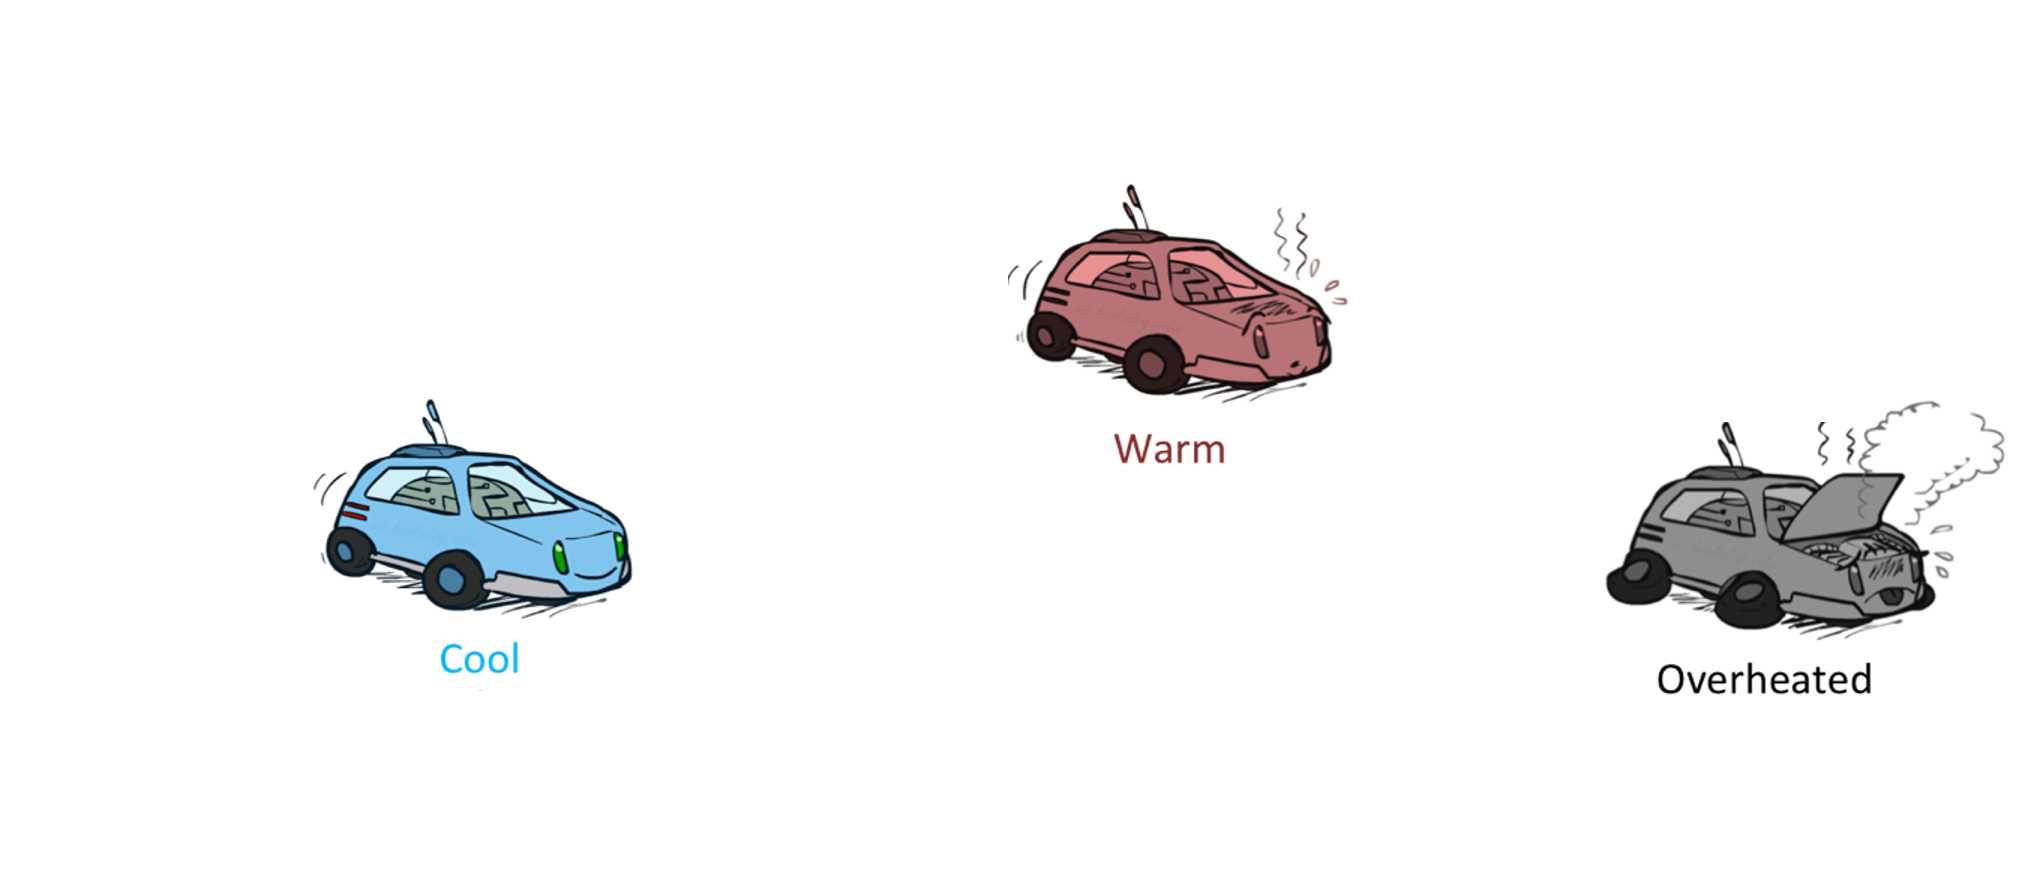
\includegraphics[width=0.8\textwidth]{L9/RL1}
   \end{textblock*}
  \end{frame}
  
  
  \begin{frame}{Offline (MDPs) vs. Online (RL)}
   \begin{columns}
    \begin{column}{0.5\textwidth}
     \begin{center}\scriptsize
      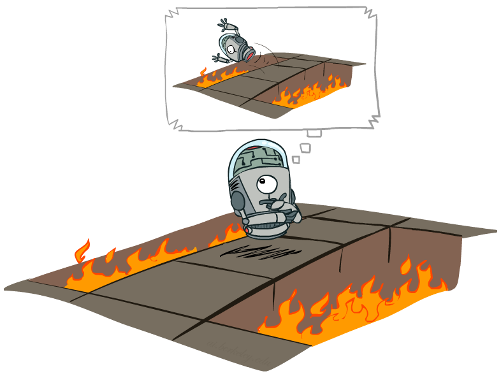
\includegraphics[width=0.9\textwidth]{L9/offline}\\[1em]
      Offline solution
     \end{center}
    \end{column}
    \begin{column}{0.5\textwidth}
    \vspace{3.8em}
     \begin{center}\scriptsize
      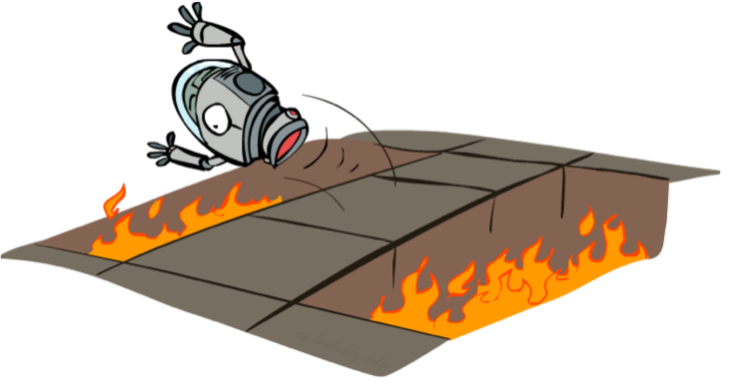
\includegraphics[width=0.9\textwidth]{L9/online}\\[1em]
      Online solution
     \end{center}
    \end{column}
   \end{columns}
  \end{frame}
  
  
  \begin{frame}{Why Not Use Policy Evaluation?}
   \begin{itemize}[<+->]
   \setlength{\itemsep}{1.2em}
    \item Simplified \alert{Bellman updates} calculate V and Q for a fixed policy
    $$V^\pi_{t}(s) \leftarrow \sum_{s^\prime}p(s, \pi(s), s^\prime) \left(r(s, \pi(s), s^\prime) + \delta V^\pi_{t-1}(s^\prime)\right)$$
    \item This approach fully exploited connections between the states
    \item Unfortunately, we need $p$ and $r$ to do it!
   \end{itemize}
  \end{frame}
  
  
  \begin{frame}{Temporal Difference (TD) Learning}
   \begin{itemize}[<+->]
   \setlength{\itemsep}{0.7em}
    \item Main idea: learn from every experience!
    \begin{itemizes}[0.5em]
     \item Update $V(s)$ each time we experience a transition $(s, a, s^\prime, r)$
     \item Likely outcomes $s^\prime$ will contribute updates more often
    \end{itemizes}
    \item Temporal difference learning of values
    \begin{itemizes}[0.5em]
     \item Policy still fixed, still doing evaluation!
     \item Move values toward value of whatever successor occurs: running average
     \begin{eqnarray*}
     &\text{Sample of }V(s): & r(s, a, s^\prime) + \delta V^\pi(s^\prime)\\[0.5em]
     &\text{Update of }V(s): & V^\pi(s) \leftarrow (1-\alpha)V^\pi(s) + \alpha \left(r(s, a, s^\prime) + \delta V^\pi(s^\prime)\right)\\[0.5em]
     &\text{Same update}: & V^\pi(s) \leftarrow V^\pi(s) + \alpha \left(r(s, a, s^\prime) + \delta V^\pi(s^\prime) - V^\pi(s)\right)
     \end{eqnarray*}
    \end{itemizes}
   \end{itemize}
  \end{frame}
  
  
  \begin{frame}{Problems with TD Value Learning}
   \begin{itemize}
   \setlength{\itemsep}{1em}
    \item TD value leaning is model-free way to do policy evaluation
    \item It mimics Bellman updates with running sample averages
    \item However, if we want to turn values into (new) policy, we need $p$ and $r$!
    \begin{eqnarray*}    
     \pi(s) & = &\underset{a}{\argmax} \; Q(s, a)\\
     Q^\pi(s,a) & = &\sum_{s^\prime}p(s, a, s^\prime) \left(r(s, a, s^\prime) + \delta V(s^\prime)\right)
    \end{eqnarray*}
    \item To solve this, we can learn Q-values instead of values
    \item This makes action selection model-free too!
   \end{itemize}
  \end{frame}
  
  
  \begin{frame}{Active Reinforcement Learning}
   \begin{center}
    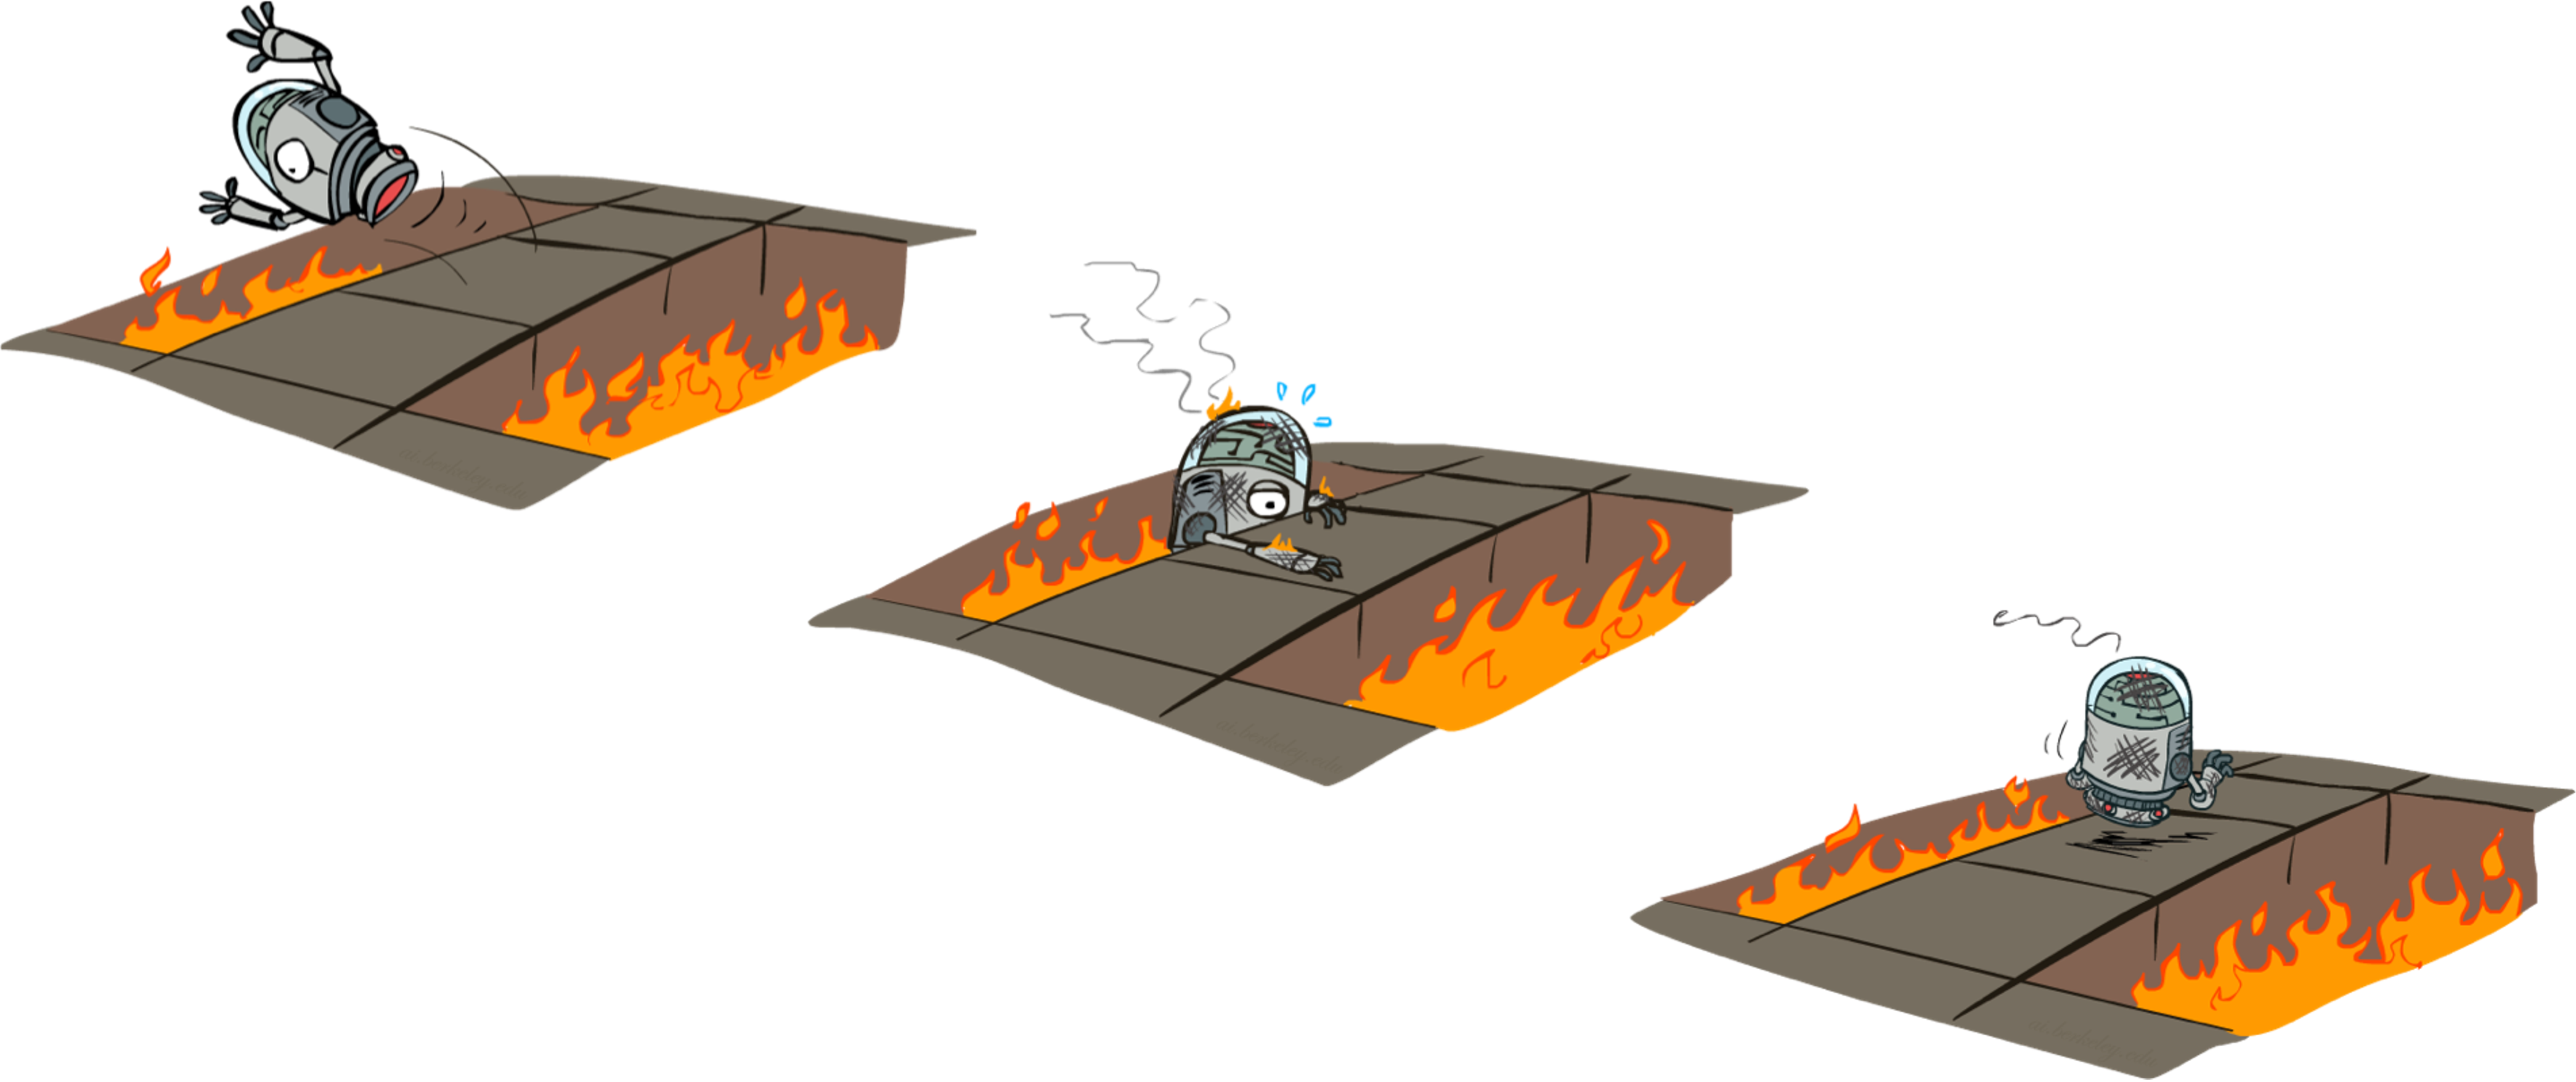
\includegraphics[width=0.85\textwidth]{L9/active}
   \end{center}
  \end{frame}
  
  
  \begin{frame}{Q-learning}
   \begin{itemize}[<+->]
    \item Q-Learning is sample-based Q-value iteration
    $$Q_{t}(s, a) \leftarrow \sum_{s^\prime}p(s, a, s^\prime) \left(r(s, a, s^\prime) + \delta \; \underset{a^\prime\in A}{\max} \; Q_{t-1}(s^\prime, a^\prime)\right)$$
    \item We learn $Q(s,a)$ values as we go
    \begin{eqnarray*}
     &\text{Sample}: & r(s, a, s^\prime) + \delta \; \underset{a^\prime\in A}{\max} \; Q(s^\prime, a^\prime)\\[0.5em]
     &\text{Update}: & Q(s,a) \leftarrow (1-\alpha_t)Q(s,a) + \alpha_t \left(r(s, a, s^\prime) + \delta \; \underset{a^\prime\in A}{\max} \; Q(s^\prime, a^\prime)\right)
    \end{eqnarray*}
   \end{itemize}
  \end{frame}
  
  
  \begin{frame}{Q-learning Algorithm}
   \begin{algorithm*}[H]
    \Repeat{until convergence}{
	 observe current state $s$\;
	 select action $a$ and take it (e.g., via \alert{$\epsilon$-greedy} policy)\;
	 observe next state $s^\prime$ and reward $r(s,a,s^\prime)$\;
	 $Q_{t+1}(s,a) \leftarrow (1-\alpha_t)Q_{t}(s,a) + \alpha_t \left(r(s, a, s^\prime) + \delta V_t(s^\prime)\right)$\;
	 $V_{t+1}(s) \leftarrow \max_a Q_t(s, a)$\;
	}
   \end{algorithm*}
   \vspace{1em}
   \begin{itemize}
    \item $\epsilon$-greedy: W.p. $\epsilon$, act randomly, w.p. $(1-\epsilon)$ act according to $Q_t$
   \end{itemize}
  \end{frame}
  
  
  \begin{frame}{Q-learning Properties}
   \begin{itemize}
   \setlength{\itemsep}{1em}
    \item Q-learning converges to optimal policy -- even if agent acts sub-optimally!
    \item This is called \alert{off-policy learning}
    \item There are some caveats
    \begin{itemizes}[0.7em]
     \item We have to explore enough
     \item We have to eventually make the learning rate small enough
     \item But we should not decrease it too quickly
     \item Q-learning converges if $\sum_0^\infty \alpha_t = \infty$ and $\sum_0^\infty \alpha^2_t < \infty$
     \item Basically, in the limit, it does not matter how you select actions (!)
    \end{itemizes}
   \end{itemize}
  \end{frame}
  
  
 \section{Multi-agent Reinforcement Learning}
  
  
  \begin{frame}{Independent Single-agent RL}
   \begin{itemize}[<+->]
   \setlength{\itemsep}{1.2em}
    \item Setting: Two-player zero-sum games
    \item Naive idea: Agents \alert{ignore} the existence of their opponent
    \item $Q_i^\pi(s,a_i)$: Value for $i$ if both agents follow $\pi$ starting from $s$ and $i$ plays $a_i$
    \item Learning dynamics: Agents deploy \alert{independent Q-learning}
    \item {\color{darkgreen}Good news}: \alert{No-regret} property if opponent plays stationary policy
    \item \alert{Bad news}: No convergence guarantee if both agents are learning (e.g., \alert{self play})!
   \end{itemize}
  \end{frame}
  
  
  \begin{frame}{Minimax-Q}
   \begin{itemize}[<+->]
   \setlength{\itemsep}{1.2em}
    \item Littman%
    \footnote{\tiny Littman, M. L. ``Markov games as a framework for multi-agent reinforcement learning.'' 1994}
    extended Q-learning algorithm to zero-sum stochastic games
    \item Main idea is to modify $Q$-function to consider actions of opponent
    $$Q_{i,t+1}(s_t, a_t) = (1 - \alpha_t)Q_{i,t}(s_t, a_t) + \alpha_t\left(r_i(s_t,a_t) + \delta V_{i,t}(s_{t+1})\right)$$
    \item Since game is zero sum, we can have
    $$V_{i,t}(s) = \underset{\pi_i}{\max} \; \underset{a_{-i}}{\min}\; Q_{i,t}(s,\pi_i,a_{-i})$$
   \end{itemize}
  \end{frame}
  
  
  \begin{frame}{Minimax-Q Algorithm}
   \begin{algorithm*}[H]
    \Repeat{until convergence}{
	 observe current state $s$\; \pause
	 select action $a_i$ and take it (e.g., via \alert{$\epsilon$-greedy} policy)\; \pause
	 observe action profile $a$\; \pause
	 observe next state $s^\prime$ and reward $r(s,a,s^\prime)$\; \pause
	 $Q_{i,t+1}(s,a) \leftarrow (1-\alpha_t)Q_{i,t}(s,a) + \alpha_t \left(r(s, a) + \delta V_{i,t}(s^\prime)\right)$\; \pause
	 $\pi_i(s,\cdot) \leftarrow \argmax_{\pi^\prime} \min_{a_{-i}} \sum_{a_i} \pi^\prime(s,a_i) Q_{i,t}(s,a_i,a_{-i})$\; \pause
	 $V_{t+1}(s) \leftarrow \min_{a_{-i}} \sum_{a_i} \pi(s,a_i) Q_{i,t}(s,a_i,a_{-i})$\;
	}
   \end{algorithm*}
  \end{frame}
  
  
  \begin{frame}{Minimax-Q Algorithm: Discussion}
   \begin{itemize}
   \setlength{\itemsep}{1.2em}
    \item It guarantees agents payoff at least equal to that of their maxmin strategy
    \item In zero-sum games, minimax-Q converges to the value of the game in self play
    \item It no longer satisfies no-regret property
    \item If opponent plays sub-optimally, minimax-Q does not exploit it in most games
   \end{itemize}
  \end{frame}
  
  
  \begin{frame}{Nash-Q}
   \begin{itemize}
   \setlength{\itemsep}{1em}
    \item Hu and Wellman%
    \footnote{\tiny Hu, J, and Wellman, M. P. ``Multiagent reinforcement learning: theoretical framework and an algorithm." 1998}
    extended minimax-Q to general-sum games
    \item Algorithm is structurally identical to minimax-Q
    \item Extension requires that each agent maintains values for all other agents
    \item LP to find maxmin value is replaced with quadratic programming to find NE
    \item Nash-Q makes number of very limiting assumptions (e.g., uniqueness of NE)
   \end{itemize}
  \end{frame}
  
  
  \begin{frame}{Recall: Stochastic Games Model}
   \begin{itemize}[<+->]
   \setlength{\itemsep}{1.2em}
    \item Focus on \alert{stationary Markov strategies} (a mixed strategy per state)
    \item $\pi_i: S \mapsto \Delta(A_i)$ denotes (mixed) strategy of agent $i$ at state s 
    \item $\pi = (\pi_1,\dots,\pi_n)$ denotes strategy profile of all agents
    \item \alert{Expected utility (value) function} of agent $i$ is
    $$v_i(s,\pi) \defeq \E_{a_k\sim \pi(s_k)}\left[\sum_{k=0}^{\infty}\delta^k r_i(s_k,a_k)\given s_0 = s\right]$$
   \end{itemize}
  \end{frame}
  
  
  \begin{frame}{Equilibrium Characterization}
   \begin{itemize}[<+->]
    \item Equilibrium \alert{value function} is defined using \alert{one-stage deviation} principle (\alert{multi-agent} extension of \alert{Bellman's equation}) as
    $$v_i(s,\pi^*) = \underset{\pi_i}{\max}\;\E_{a\sim (\pi_i,\pi_{-i}^*(s))}\left[r_i(s, a) + \delta \sum_{s^\prime\in S}p(s, a, s^\prime) v_i(s^\prime, \pi^*)\right]$$
    \item \alert{Q-function} is defined as
    $$Q_i(s,a,\pi^*) = r_i(s, a) + \delta \sum_{s^\prime\in S}p(s, a, s^\prime) v_i(s^\prime, \pi^*)$$
    \item Recursion is then defined as
    $$v_i(s, \pi^*) = \underset{\pi_i}{\max}\;\E_{a\sim (\pi_i,\pi_{-i}^*(s))}\left[Q_i(s,a,\pi^*)\right]$$
   \end{itemize}
  \end{frame}
  
  
  \begin{frame}{FP for Model-based Learning}
   \begin{itemize}[<+->]\small
   \setlength{\itemsep}{1em}
    \item Consider learning dynamic that combines FP with value-function (or Q-function) iteration
    \item Agents form beliefs on opponent strategies (using empirical frequencies and assuming opponent uses stationary strategy)
    \item Agents also form beliefs about \alert{equilibrium} value function, or Q-function
    \item Agents then choose best response action in \alert{auxiliary game} given their beliefs (where payoffs are given by Q-function estimates)
    \item Key challenge is that payoffs or value functions in these auxiliary games are \alert{non-stationary} (unlike repeated play of stage games)
   \end{itemize}
  \end{frame}
  
  
  \begin{frame}{FP for Model-based Learning: Model}
   \begin{itemize}[<+->]\small
    \item At time $t$, $i$'s belief on $-i$'s strategy is $\mu^t_{i}$ and on own Q-function is
    $$Q_i^t \defeq \E_{a_{-i}\sim \mu_{i}^t(s)}[Q_i^t(s,a_i,a_{-i})]$$
    \item Agent $i$ selects best response $a^t_i(s) \in \argmax_{a_i} Q_i^t(s,a_i,\mu_{i}^t(s))$
    \item Agent $i$ updates $\mu_i$ as 
    $$\mu_i^{t+1}(s) = (1-\alpha_t)\mu_i^t(s) + \alpha_t a_{-i}^t(s)$$
    \item Agent $i$ updates $Q_i$ as
    $$Q_i^{t+1}(s,a) = (1-\beta_t)Q_i^t(s,a)+\beta_t\left(r_i(s, a) + \delta \sum_{s^\prime\in S}p(s, a, s^\prime) v_i^t(s^\prime)\right)$$
    where $v_i^t(s^\prime) = \max_{a_i}Q_i^t(s^\prime,a_i,	\mu_i^t(s))$
   \end{itemize}
  \end{frame}
  
  
  \begin{frame}{Two-timescale Learning Framework}
   \begin{itemize}[<+->]\small
   \setlength{\itemsep}{1.2em}
    \item Beliefs on Q-functions are updated at slower rate than beliefs on opponent strategies
    \item This postulate agents' choices to be more dynamic than changes in their preferences
    \item Q-functions in auxiliary games can be viewed as slowly evolving agent preferences
    \item This enables weakening the dependence between evolving strategies and Q-functions
   \end{itemize}
  \end{frame}
  
  
  \begin{frame}{Convergence of Two-timescale Learning Framework}
   \begin{itemize}
   \setlength{\itemsep}{1em}
    \item If each state is visited \alert{infinitely} many times
    \item And, if $\lim_{k\to \infty} \alpha_k = \lim_{k\to \infty} \beta_k = 0$ and $\sum_k \alpha_k = \sum_k \beta_k = \infty$
    \item And, if $\lim_{k\to \infty} \beta_k / \alpha_k = 0$ (two-timescale learning: $\beta_k \to 0$ faster than $\alpha_k \to 0$)
    \item Then $Q$ and $\mu$ converge to NE value and strategy in zero-sum stochastic games
    \item They also converge to NE value for single-controller stochastic games
   \end{itemize}
  \end{frame}
  

  \begin{frame}{Acknowledgment}
   \begin{itemize}
    \setlength{\itemsep}{1em}
    \item This lecture is a slightly modified version of ones prepared by
    \begin{itemizes}
     \item Asu Ozdaglar \href{https://ocw.mit.edu/courses/electrical-engineering-and-computer-science/6-254-game-theory-with-engineering-applications-spring-2010/index.htm}{[MIT 6.254]}
     \item Vincent Conitzer \href{https://courses.cs.duke.edu/spring16/compsci590.4/}{[Duke CPS 590.4]}
     \item Aaron Roth \href{https://www.cis.upenn.edu/~aaroth/courses/agtS21.html}{[UPenn NETS 412]}
     \item Dan Klein and Pieter Abbeel \href{http://ai.berkeley.edu/home.html}{[UC Berkeley CS 188]}
    \end{itemizes}
   \end{itemize}
  \end{frame}
  
  
\end{document}
